\section {Numerical Example}
\subsection {Multi-Resolution Analysis in One Dimension}

\begin{figure}
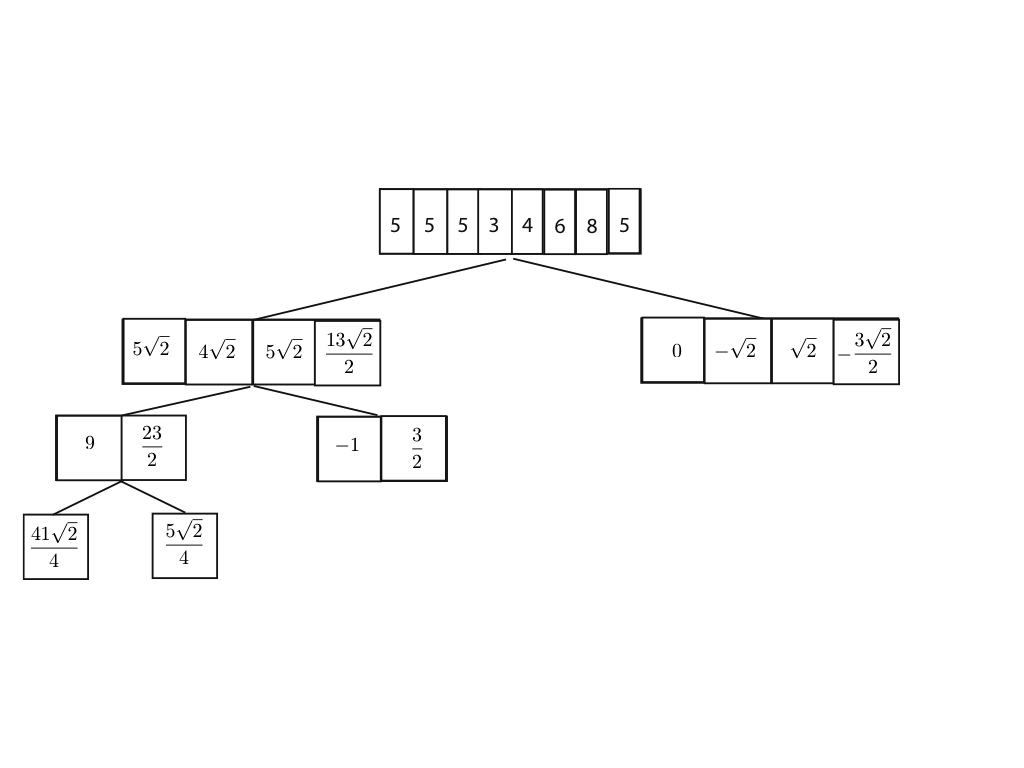
\includegraphics [width=7in]{mraexample.jpg}
\caption{The Haar Transform performed a sample function show each step of the transform in multi-resolution analysis }
\label{nummra}
\end{figure}

\begin{figure}
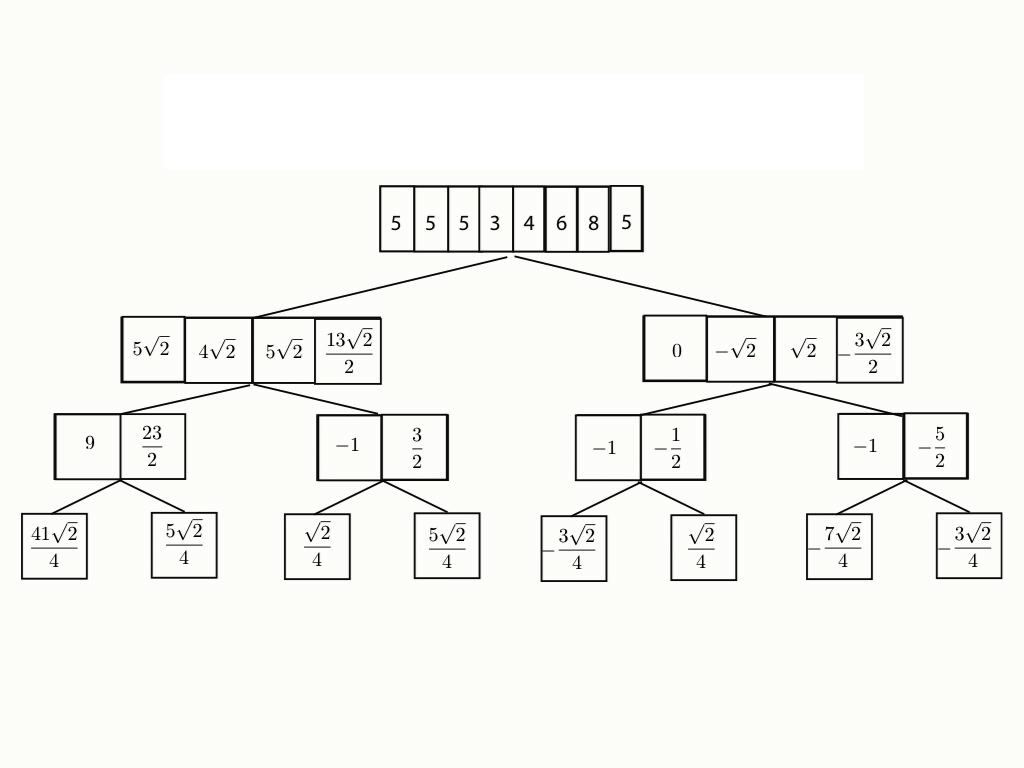
\includegraphics [width=7in]{numexample01.jpg}
\caption{The Haar Transform performed a sample function show each step of the transform in multi-resolution expansion }
\label{nummre}
\end{figure}

MRA starts with the original array.  The wavelet transform is applied to the array.   After the first application of the wavelet transform, an average and difference array now exist.  This is shown in figure %\cite{} 
as the first two children in what is called here as a wavelet binary tree.

For MRA, the analysis is continued on the average branch.  The difference branch ignored.  This procedure is repeated on the average branch.   The stopping point is determined by the size of array.  There exist formulae that defines this finite limit.  
\[\max_n(\gcd(2^n,S)) \]  
where 
\begin{itemize}
\item $n$ is the finite limit
\item $s$ is the size

\end{itemize}

Once completed, the arrays are joined into an array which is the same size as the original.  The energy is generally concentrated at the beginning of the array.  Also, the energy of the array tends to be ordered from strongest to weakest.  Terms representing change are kept as pairs to each section.  

There is an analogues in time and frequency domain.  As the MRA is applied, the lower frequencies further isolated.  The different branches represents a band pass filter with ranges 
\[ [\frac{\pi}{2^l} , \frac{\pi}{2^{l-1}} ] \]
where $l$ is the level in wavelet tree where the difference branch is.  

\subsection {Multi-Resolution Expansion in One Dimension}
Like MRA, MRE starts with an original array, and applies a wavelet transform to that array.  The decomposition is also represented by binary tree, with an average and difference branch.  The limit and height of the tree is also the same:
\[\max_n(\gcd(2^n,S)) \]  
where 
\begin{itemize}
\item $n$ is the finite limit
\item $s$ is the size

\end{itemize}

What is not the same is how the wavelet transform is reapplied.  In addition to being applied on the average branch again,  but the wavelet transform is also applied to the difference branch also.   An example is provided in Figure %\cite{}. 
The sub arrays are reinserted into the array in order from the left branch to the right branch.  

In the time and frequency analogues, each transformation filters the array with high pass and low pass filter.  The frequency width of these sub arrays is proportional to length of the original array.  The center frequency is relative to the position of the sub-array within the array.   The lowest frequency components are on the average side of the array, and the highest frequency components are on the difference section of the array.  One special case exists for arrays of length $2^n$.  If the array is of length $2^n$ then the full MRE yields entire frequency domain.  In case that the array is of odd size larger than one, then no transform can be applied and contains only time domain information.  When the length of the array is of $c\cdot 2^n$ where $c$ is an odd integer larger than one, then the full decomposition contains both positional and frequency information.  

  
\subsection {$\psi^n$ Expansion in One Dimension}
One other form of the multi-resolution expansion that can be used is almost trivial by its nature, $\psi^n$ expansion.  This particular form has the same branches as the MRE.  However, the sub arrays are place back in the array in a different order.    Figure illustrates the difference in ordering from the $\psi^n$ form and the MRE form.    This form makes for analysis such time and frequency difficult, but contributes advantages linear operations.
